\documentclass[justified, nobib]{tufte-handout}

\usepackage{Haust2017almennt}

\title{Stærðfræðimynstur í tölvunarfræði  \semester - Námsáætlun og upplýsingar}

\begin{document}

\section{Námsáætlun}
\label{sec:schedule}

Námskeiðið er grundvallarnámskeið í strjálli stærðfræði, sérstaklega ætlað nemendum í tölvunarfræði og hugbúnaðarverkfræði. 
Sömuleiðis getur námskeiðið veitt nemendum á öðrum námslínum kynningu á helstu stærðfræðihugtökum sem endurtekið koma við sögu í tölvunarfræði.

\begin{table*}
\caption{Námsáætlun eftir vikum}
\label{tab:schedule}
\begin{center}
\begin{tabularx}{\linewidth}{lccXp{3cm}}
\toprule
&\multicolumn{2}{c}{Dagsetningar}&&\\
\cmidrule{2-3}
Vika&Þri&Fös&Námsefni&Kaflar\\
\midrule
1	&22/8	&25/8	& Kynning á námskeiðinu, rök, \LaTeX                                                                    &1.1-1.4\\
2	&29/8	&1/9	& Sannanir, mengi, föll                                                                                 &1.7-1.8, 2.1-2.3\\
3	&5/9	&8/9	& Runur, fjöldatölur, fylki, reiknirit                                                                  &2.4-2.6, 3.1\\
4	&12/9	&5/9	& Vöxtur falla, tímaflækjur                                                                             &3.2-3.3\\
5	&19/9	&22/9	& Heiltölureikningar, leifar, rökstudd forritun                                                         &4.1-4.4, 5.5\\
6	&26/9	&29/9	& Dulkóðun, þrepun                                                                                      &4.6, 5.1\\
7	&3/10	&6/10	& Talning, skúffureglan, umraðanir og samantektir                                                       &6.1-6.4\\
8	&10/10	&13/10	& Vensl, venslaaðgerðir, vensl í gagnagrunnum                                                           &9.1-9.3\\
9	&17/10	&20/10	& Endurkvæmni, rakningarvensl, deila-og-drottna reiknirit                                               &5.3, 8.1-8.3\\
10	&24/10	&27/10	& Net, mismunandi gerðir neta, framsetning neta                                                         &10.1-10.3\\
11	&31/10	&3/11	& Euler-vegir, Hamilton-vegir, stysta-vegs vandamál                                                     &10.4-10.6\\
12	&7/11	&10/11	& Lagnet, hnútalitanir, tré, hagnýtingar á trjám, trjáflakk                                             &10.7-10.8, 11.1-11.3\\
13	&14/11	&17/11	& Spanntré, endanlegar stöðuvélar                                                                       &11.4-11.5, 13.3\\
14	&21/11	&24/11	& Turing-vélar, upprifjun                                                                               &13.5\\
\bottomrule
\end{tabularx}
\end{center}
\end{table*}

Þar með er áætlað að eftirfarandi kaflar og undirkaflar mæti afgangi: 1.6-1.7, 4.5, 5.2, 6.5-6.6, allur kafli 7, 8.4-8.6, 9.4-9.6, allur kafli 12, 13.1-13.2 og 13.4.

\section{Kennari}
Aðalkennari er Eiríkur Ernir Þorsteinsson. Aðsetur er í Tæknigarði, 2. hæð, stofa 214. Sjá mynd \ref{fig:taeknigardur}.

\begin{marginfigure}
\caption{Önnur hæð í Tæknigarði}
\label{fig:taeknigardur}
\begin{center}
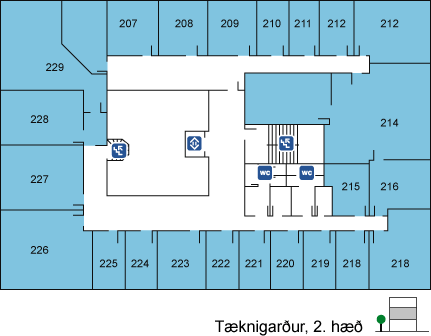
\includegraphics[width=\linewidth]{taeknigardur}
\end{center}
\end{marginfigure}

Til að hafa samband við kennara er ráðlagt að setja inn þráð á \href{piazza.com/hi.is/fall2017/tl104g/home}{Piazza}. Allar fyrirspurnir sem ekki fela í sér persónulegar upplýsingar ættu að fara þangað. Tölvupóstfang er \href{mailto:ernir@hi.is}{ernir@hi.is}.

Ef um veikindi, námsörðugleika eða áföll er að ræða skal hafa samband við Náms- og starfsráðgjöf HÍ, sjá \nameref{sec:help} hér að neðan.
\section{Tímar og námstilhögun}
Aðalkennsla fer fram í fyrirlestrum. Fyrirlestrarnir eru á þriðjudögum klukkan 15:00 og föstudögum klukkan 8:20 í stofu HT-105\footnote{Undantekning: Fyrsti fyrirlesturinn, 22. ágúst. Sjá Uglu.}.

Dæmatímar eru á þriðjudögum og miðvikudögum. Nemendum er frjálst að mæta í þá dæmatíma sem henta best.\footnote{Kennari mun skerast í leikinn ef sókn í dæmahópana verður mjög ójöfn.}

Ekki er skylda að mæta í fyrirlestra eða dæmatíma. Nemendur eru ábyrgir fyrir því að forgangsraða tíma sínum.
\subsection{Upptökur á fyrirlestrum}
Fyrirlestrar eru teknir upp þegar tæknin leyfir.  Upptökurnar verða gerðar með Panopto og aðgengilegar í gegnum Uglu. Varað er við því að treysta á upptökur í stað mætingar í fyrirlestra þar sem upptökur geta brugðist og upplifunin er ekki sú sama.
\subsection{Álag}
Námskeiðið er $8 ECTS$ einingar. 60 ECTS einingar eru skilgreindar sem 1500-1800 klst. af vinnu.
\[
    \text{60 ECTS = 1650 klst.} \Longleftrightarrow \text{8 ECTS = 220 klst.}
\]
Misserið er 14 vikur, svo gera má ráð fyrir 15-16 klst. af vinnu í viku. Þar af eru 4 klst. í fyrirlestrum og dæmatímum.
\section[Bók]{Bók og stuðningsefni}
\label{sec:book}
Kennslubók er \emph{Discrete Mathematics and its Applications}, sjöunda útgáfa, eftir Rosen. Bókinni fylgir stuðningsefni, sjá \nameref{sec:tools}.

\begin{marginfigure}
    \caption{Sjöunda útgáfa kennslubókarinnar}
    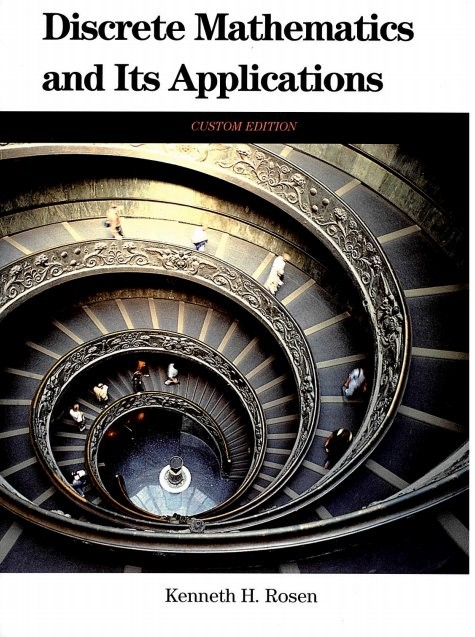
\includegraphics[width=\linewidth]{Pics/rosen}
\end{marginfigure}

Nokkrar leiðir eru til að nálgast kennslubók og tilheyrandi efni:
\begin{itemize}
    \item Kaupa bók úr pappír (fæst í Bóksölu stúdenta), vefbók og æfingaaðgangur fylgir með
    \item Kaupa vefbók og æfingaaðgang á vefsíðu
    \item Kaupa æfingaaðgang eingöngu
\end{itemize}
Eldri útgáfur bókarinnar innihalda að miklu leyti sama efni, en líklegt er að dæmi hafi breyst eða númer þeirra riðlast.

\section{Námsmat, einkunnir og próf}
\subsection{Netæfingar/Dæmatímadæmi}
Æfingar á Connect kerfinu (sjá \nameref{sec:tools}) verða lagðar fyrir í hverri viku, ætlaðar til vinnu í dæmatímum. Vægi þeirra er 10\% af lokaeinkunn. Þátttaka í $n$ netæfingum gefur hluteinkunnina $n$, að hámarki 10.

\subsection{Skilaverkefni}
\begin{marginfigure}
    \caption{Samsetning lokaeinkunnar}
    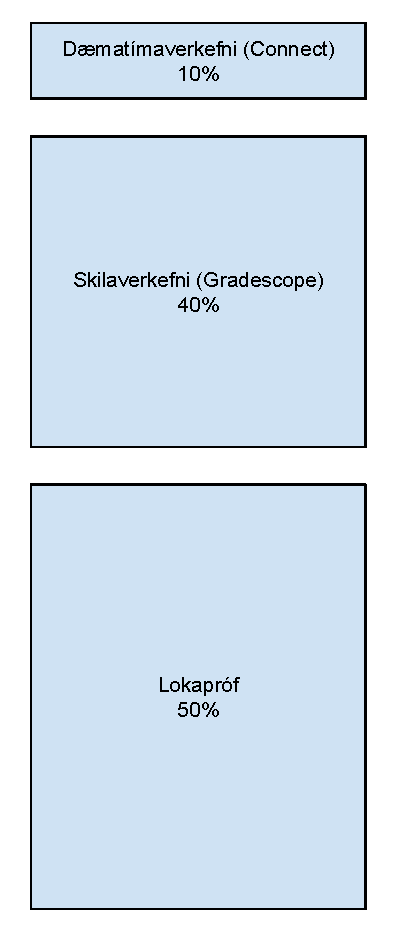
\includegraphics[width=\linewidth]{Pics/namsmat}
\end{marginfigure}
Vikuleg verkefnaskil eru í námskeiðinu. Meðaleinkunn 10 bestu skilaverkefnanna er 40\% af lokaeinkunn. Verkefnunum skal skila á Gradescope.com (sjá \nameref{sec:tools}). Athugið að \textbf{ekki er tekið við skilum eftir að Gradescope lokar}.

Nauðsynlegt er að skila fjórum af fyrstu sex skilaverkefnunum til að öðlast próftökurétt.
\subsection{Próf}
Vægi lokaprófs er 50\% af lokaeinkunn. Leyfilegt verður að taka með eitt blað af glósum (skrifað á báðar hliðar) í prófið.

Lágmarkseinkunn er 5. Nauðsynlegt er að ná lágmarkseinkunn á lokaprófi sem og í námskeiðinu sem heild til að standast námskeiðið.
\section{Kennslutól}
\label{sec:tools}
Ýmis verkennslutól verða notuð. Mælt er með að nemendur skrái sig inn á eftirfarandi þjónustur sem allra fyrst:
\begin{itemize}
 \item \href{piazza.com/hi.is/fall2017/tl104g/home}{Piazza}\footnote{\url{piazza.com/hi.is/fall2017/tl104g/home}} er fyrirspurnavefurinn sem notaður er í námskeiðinu. Skráningin í námskeiðið á að vera sjálfvirk, en hafi það misfarist á að vera hægt að skrá sig handvirkt. \emph{Allar spurningar sem snúa að námskeiðinu ættu að fara inn á Piazza frekar en í tölvupóst}.
 \item \href{https://gradescope.com/courses/9487}{Gradescope.com}\footnote{\url{gradescope.com/courses/9487}} er vefkerfið sem notað er fyrir skilaverkefni. Nemendur þurfa að skrá sig sjálfir á þennan vef. Aðgangskóði námskeiðsins er \texttt{9N834D}. Mikilvægt er að skrá sig á Gradescope með fullu nafni (íslenskir stafir eru leyfilegir) og með því að nota HÍ-netfang. Kerfið tekur við \texttt{.pdf} skrám.
 \item \href{http://connect.mheducation.com/class/tol104g17}{McGraw-Hill Connect}\footnote{\url{connect.mheducation.com/class/tol104g17}} er æfingavefurinn sem notaður verður í dæmatímaverkefnum. Athugið að kaupa þarf aðgang! (Fylgir með \nameref{sec:book})
\end{itemize}

\section{Heilræði og aðstoð}
Sem og í öðrum háskólanámskeiðum er virkni í námskeiðinu lykill að velgengni. Þar er helst átt við að mæta og taka þátt í tímum\footnote{Það að horfa á upptöku gerir ekki sama gagn!} og gera dæmin sem sett eru fyrir.

Skilaverkefnin eru sérstaklega mikilvæg. Það að taka sér góðan tíma í að kljást við þau er mikið lykilatriði. Þau eiga ekki að vera kvöð til að ljúka af, fyrir flestum eru það verkefnin sem virkilega fá færnina til að síast inn.
\subsection{Aðstoð}
\label{sec:help}
Mikilvægt er að gera sér grein fyrir því hvenær tími er kominn til að leita sér aðstoðar. Mikill meirihluti nemenda þarf aðstoð af einhverju tagi í hverju námskeiði.

Hægt er að fá flestum spurningum sem tengjast námskeiðinu og verkefnunum svarað á Piazza. Betra er að spyrja fyrr en seinna, áður en of mikill tími fer til spillis. Dæmatímakennarar og aðrir lengra komnir nemendur eru líka alltaf allir af vilja gerðir til að hjálpa.

\href{http://www.hi.is/verkfraedi\_og\_natturuvisindasvid/nemendathjonusta\_von}{Nemendaþjónusta VoN}\footnote{\url{hi.is/verkfraedi_og_natturuvisindasvid/nemendathjonusta_von}} getur aðstoðað við allt sem viðkemur námsferlum, uppbyggingu náms og vali á námskeiðum. Nemendaþjónustan hefur aðsetur í Tæknigarði og er mjög aðgengileg.

Ef þörf er á sérstökum úrræðum eða undanþágum skal hafa samband við \href{http://nshi.hi.is/}{Náms- og starfsráðgjöf HÍ}\footnote{\url{nshi.hi.is}}. Hægt er að leita til hennar með öll persónuleg mál sem snúa að náminu.

\end{document}